% Chapter 7

\chapter{The KIR Gene Cluster and HTLV-I}
\label{Chapter7}
\lhead{Chapter 7. \emph{The KIR Gene Cluster and HTLV-I}}

\section{Introduction}

Natural killer (NK) cells are critical components of the innate immune system that have direct involvement in the anti-viral immune response \citep{Biron1999}. In addition to direct cytotoxic and antiviral functions, they have the potential to interact with components of the adaptive immune system, including T cells and dendritic cells \citep{Raulet2004}. This interaction implies a broad role in immunity and potential involvement in a wide range of diseases, including infections, cancers, and autoimmune disorders. NK cells are controlled by many activating and inhibitory receptors \citep{Lanier2005,Colucci2002}. In humans, one of the key receptor families contributing to the NK cell receptor repertoire is the killer cell immunoglobulin (Ig)-like receptor (KIR) family. They were first identified by their ability to impart some specificity on natural killer (NK) cytolysis \citep{Harel-Bellan1986,Moretta1990}. Similar to many NK cell receptors, KIRs are expressed on T cells in addition to NK cells, affirming their role in adaptive immunity.

There is extensive diversity at the KIR gene locus, which stems from both its polygenic and multi-allelic polymorphism \citep{Uhrberg1997}. KIR gene expression patterns can vary clonally \citep{Valiante1997}, adding yet another layer of complexity to the system. Diversity at the locus may be the result of selection pressures, in a manner analogous to that proposed for the HLA class I loci. Overall, however, KIR genes can be classified as activating or inhibitory. Combinations of these genes occur to generate haplotypes with widely differing balances between activating and inhibitory types.

In this chapter, we tested the hypothesis that certain KIR-HLA associations are beneficial or detrimental regarding disease status and proviral load in HTLV-I infection. This was based on the model that KIRs synergize with HLAs to generate compound genotypes that provide different levels of activation and inhibition, which impacts viral control. 

\section{Methods}

\subsection{Database}

The Kagoshima dataset (see \sref{chapter3/kagoshima}) provided information on the presence or absence of expression of the KIR genes of \tref{chapter7/tableKirHla}.

\subsection{Tested Associations}

For each HAM/TSP patient ($n = 230$) and AC ($n = 202$) in the dataset, we tested for the presence of each KIR and its associated HLA ligand (\tref{chapter7/tableKirHla}). The total number of inhibitory and activating pairs were counted per individual and tested against proviral load separately for both HAM/TSP and AC groups.

\begin{table}[htp]
\begin{center}
\begin{tabular}{|l|l|l|l|l|l|l|l|l|}
\hline
\multicolumn{5}{|c|}{Inhibitory} & \multicolumn{4}{c|}{Activating} \bigstrut \\
\hline
2DL1 & 2DL2 & 2DL3 & 3DL1 & 3DL2 & 2DS1\footnotemark & 2DS2 & 2DS4 & 3DS1 \bigstrut \\
\hline
C02 & C01 & C01 & B08 & A03 & C02 & C01 & C04 & B08 \bigstrut[t] \\
C04 & C03 & C03 & B13 & A11 & C04 & C03 &     & B13 \\
C05 & C07 & C07 & B27 &     & C05 & C07 &     & B27 \\
C06 & C08 & C08 & B44 &     & C06 & C08 &     & B44 \\
    &     &     & B51 &     &     &     &     & B51 \\
    &     &     & B52 &     &     &     &     & B52 \\    
    &     &     & B53 &     &     &     &     & B53 \\
    &     &     & B57 &     &     &     &     & B57 \\
    &     &     & B58 &     &     &     &     & B58 \bigstrut[b] \\
\hline
\end{tabular}
\end{center}
\caption[A summary of KIR ligand specificity]{A summary of KIR ligand specificity. Each individual in the Kagoshima dataset was labelled yes/no for the expression of the KIR alleles. For both the inhibitory and activating KIRs, their respective ligands \citep{Carrington2009} are listed. The ligands are grouped according to sequence similarites. The B alleles are those that contain the Bw4 serological motif (HLA-B\superscript{Bw4}) and the C alleles are grouped according to their amino acid residue at position 80: the group C01 \ldots C08 contain asparagine at position 80 (HLA-C\superscript{Asn80}) and the C02 \ldots C06 group contain lysine (HLA-C\superscript{Lys80}).}
\label{chapter7/tableKirHla}
\end{table}

\footnotetext{The Kagoshima dataset contained no information for 2DS1.}

We also tested whether the presence of known protective KIR-HLA associations from other pathogenic infections (see \sref{chapter7/discussion}) were protective in HTLV-I infection.

\section{Results}

We found no significant relationship between the count of inhibitory HLA-KIR interactions and proviral load, for either HAM/TSP or AC groups (\fref{chapter7/figure1}; AC: $R^2 = 0.01$, $P = 0.154$. HAM/TSP: $R^2 < 0.001$, $P = 0.96$).

\begin{figure}[htp]
\centering
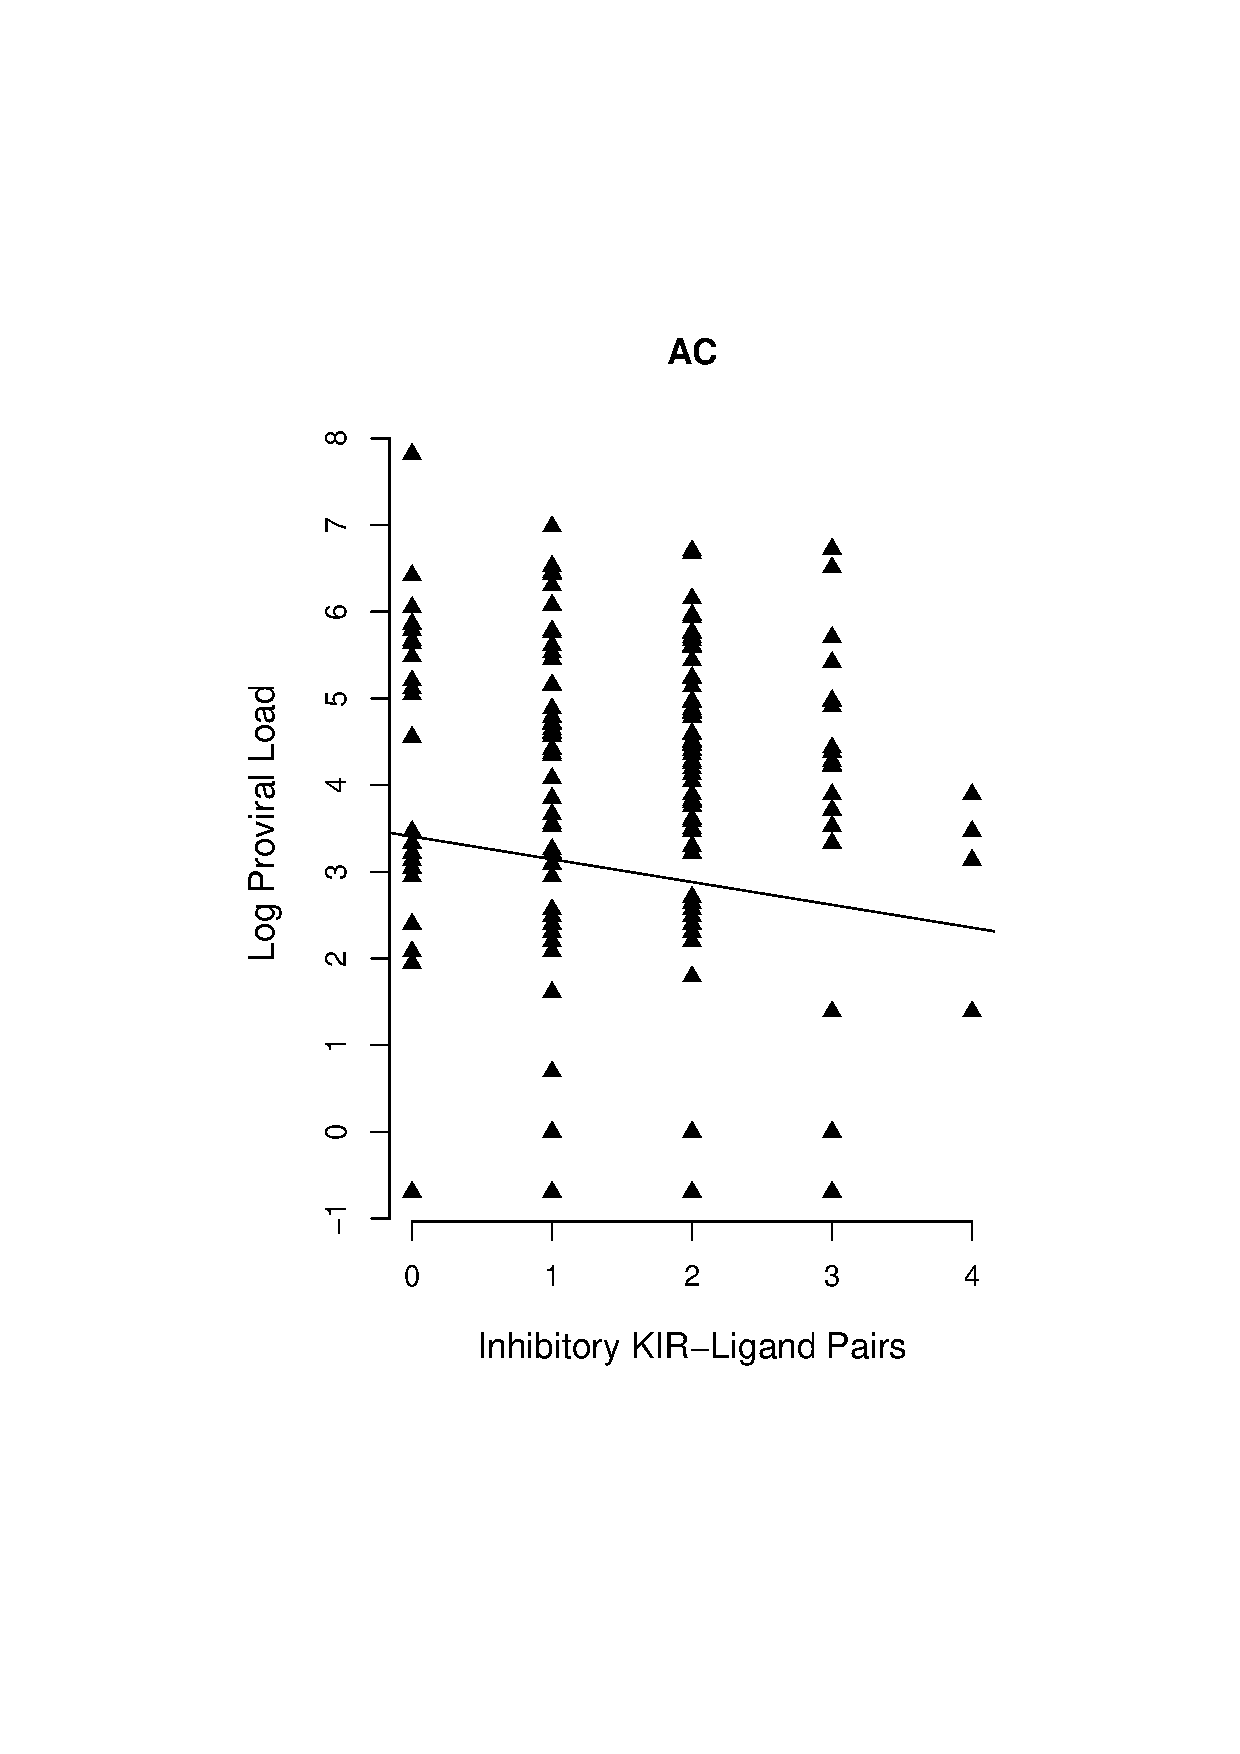
\includegraphics[width=7cm]{./Figures/chapter7/figureInhibAC}%
\hspace{0cm}%
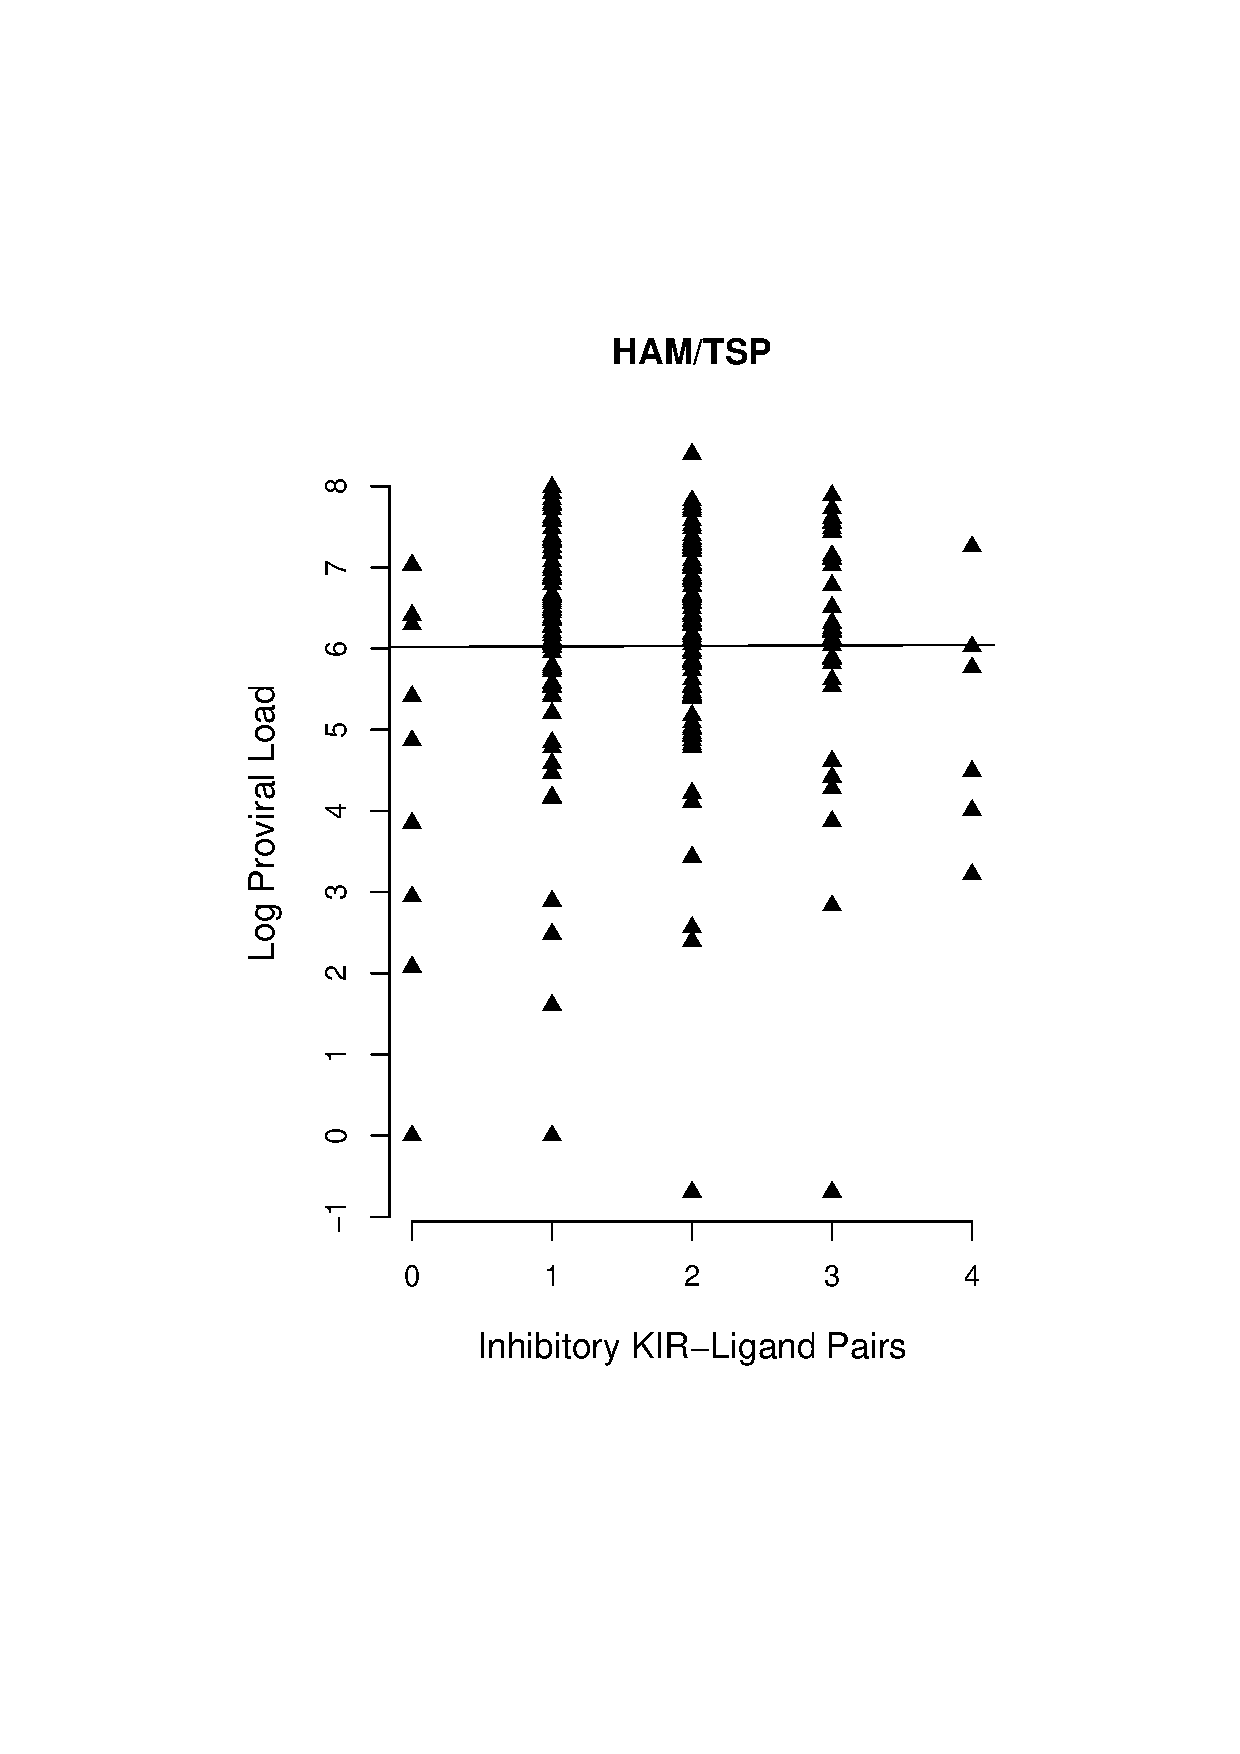
\includegraphics[width=7cm]{./Figures/chapter7/figureInhibHAM} \\
\caption[Inhibitory HLA-KIR interactions and proviral load]{The count of inhibitory HLA-KIR interactions per individual plotted against their proviral load. No significant monotonic univariate relationship was found for AC or HAM/TSP groups (AC: $R^2 = 0.01$, $P = 0.154$. HAM/TSP: $R^2 < 0.001$, $P = 0.96$).}
\label{chapter7/figure1}
\end{figure}

\fref{chapter7/figure2} shows no relationship between the count of activating KIR-HLA interactions per individual and proviral load, again for both HAM/TSP and AC groups (AC: $R^2 < 0.001$, $P = 0.867$. HAM/TSP: $R^2 = 0.003$, $P = 0.397$). We also found no relationship between the difference in activating and inhibitory KIR-HLA interactions and proviral load for the 2 groups (AC: $R^2 = 0.012$, $P = 0.117$. HAM/TSP: $R^2 = 0.002$, $P = 0.498$).

\begin{figure}[htp]
\centering
\includegraphics[width=7cm]{./Figures/chapter7/figureActivAC}%
\hspace{0cm}%
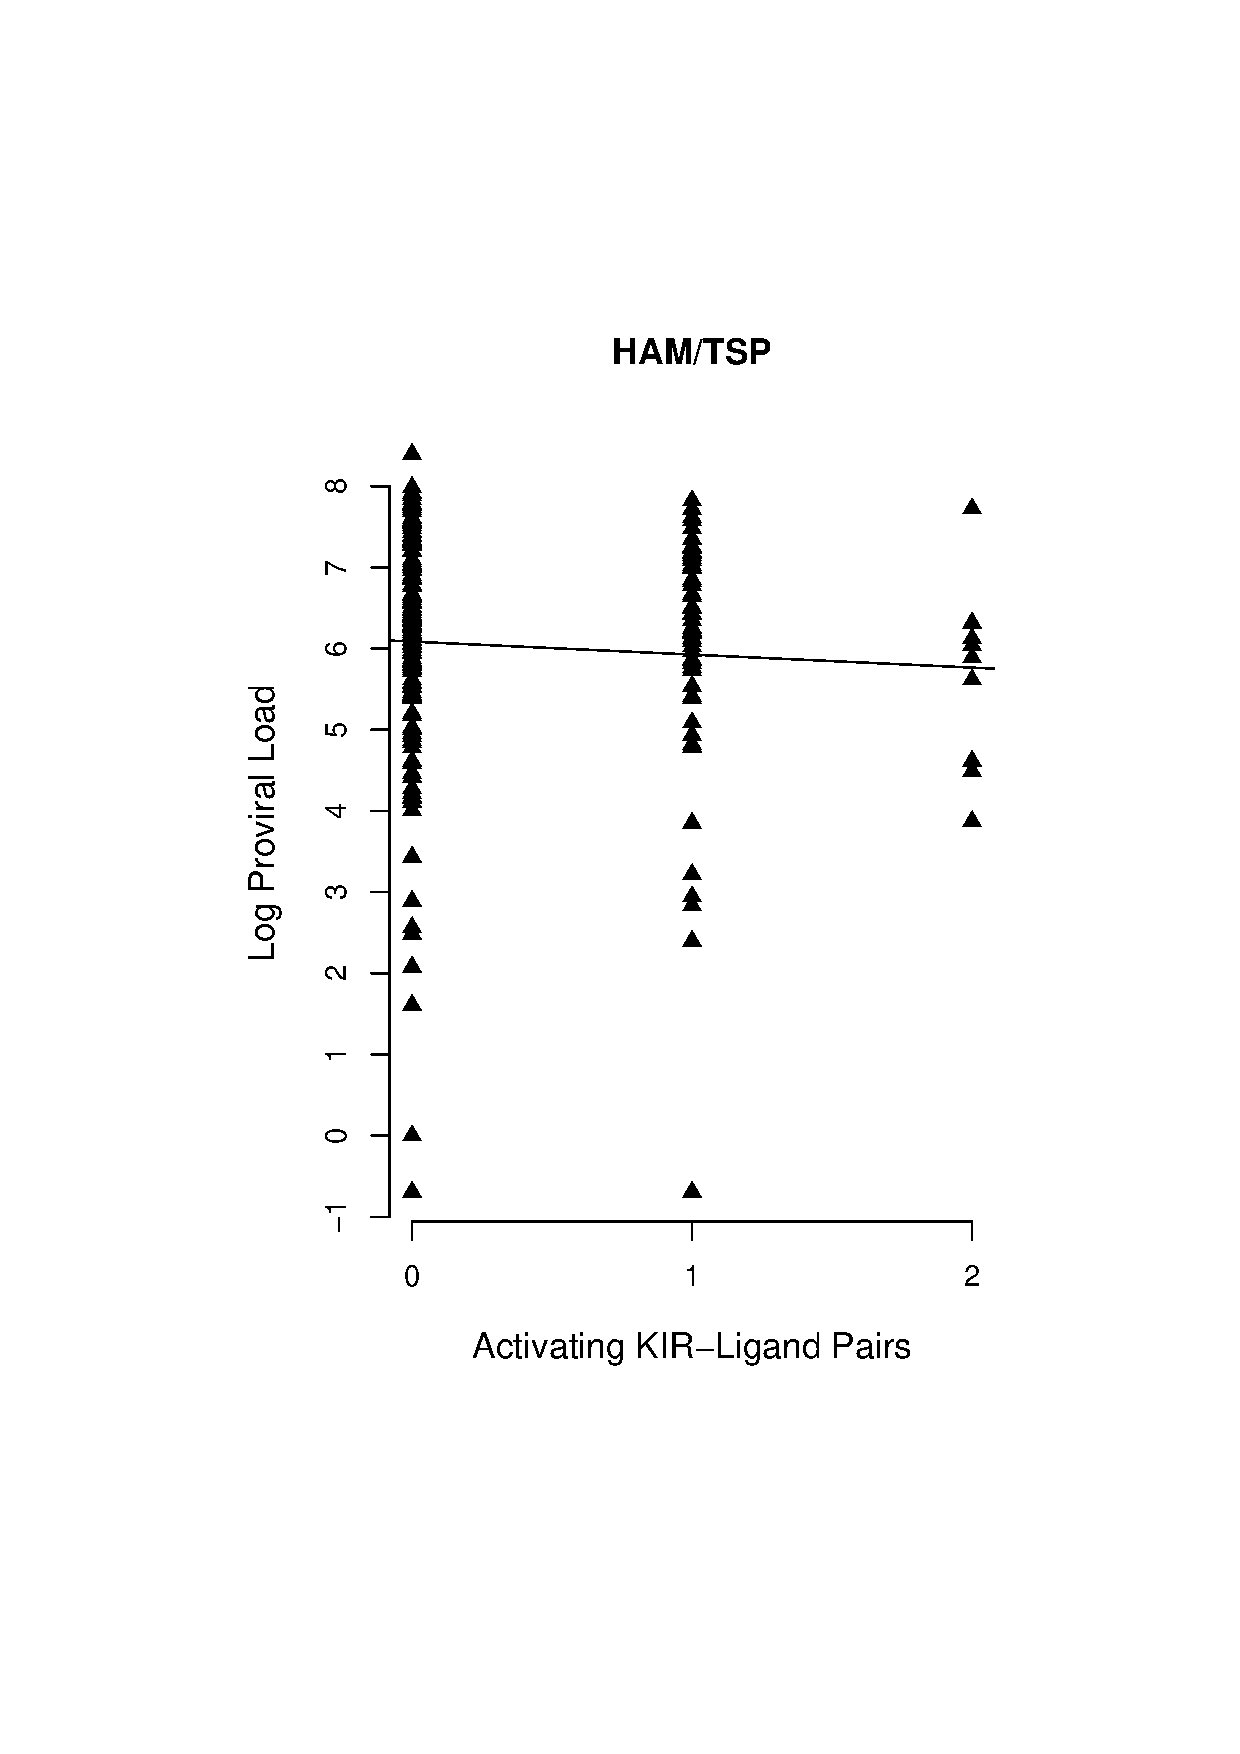
\includegraphics[width=7cm]{./Figures/chapter7/figureActivHAM} \\
\caption[Activating HLA-KIR interactions and proviral load]{The count of activating HLA-KIR interactions per individual plotted against their proviral load. No significant monotonic univariate relationship was found for AC or HAM/TSP groups (AC: $R^2 < 0.001$, $P = 0.867$. HAM/TSP: $R^2 = 0.003$, $P = 0.397$).}
\label{chapter7/figure2}
\end{figure}

\tref{chapter7/table2DL3} and \tref{chapter7/table3DS1} also demonstrate that KIR genes associated with disease outcome in other pathogens (see \sref{chapter7/discussion}) show no protective effect in terms of HTLV-I disease status (2DL3: $\chi^2 = 1.243$, $P = 0.265$. 3DS1: $\chi^2 = 0.006$, $P = 0.938$). There was no difference in proviral load between individuals expressing 2DL3 and those that did not (HAM/TSP: $P = 0.874$, AC: $P = 0.207$, Wilcoxon-Mann-Whitney). This was also the case for 3DS1 (HAM/TSP: $P = 0.393$, AC: $P = 0.289$, Wilcoxon-Mann-Whitney).

\begin{table}[htp]
\begin{center}
\begin{tabular}{|l|ll|}
\hline
 & HAM/TSP & AC \bigstrut \\
\hline
2DL3$^+$ & $n = 198$ & $n = 165$ \bigstrut[t] \\
2DL3$^-$ & $n = 32$ & $n = 37$ \bigstrut[b] \\
\hline
\end{tabular}
\end{center}
\caption[Disease risk and 2DL3]{The number of HAM/TSP and AC individuals that express KIR2DL3. There was no significant difference in the frequency of expression between the 2 groups ($\chi^2 = 1.243$, $P = 0.265$).}
\label{chapter7/table2DL3}
\end{table}

\begin{table}[htp]
\begin{center}
\begin{tabular}{|l|ll|}
\hline
 & HAM/TSP & AC \bigstrut \\
\hline
3DS1$^+$ & $n = 38$ & $n = 33$ \bigstrut[t] \\
3DS1$^-$ & $n = 192$ & $n = 169$ \bigstrut[b] \\
\hline
\end{tabular}
\end{center}
\caption[Disease risk and 2DS1]{The number of HAM/TSP and AC individuals that express KIR2DS1. There was no significant difference in the frequency of expression between the 2 groups ($\chi^2 = 0.006$, $P = 0.938$).}
\label{chapter7/table3DS1}
\end{table}

\section{Discussion}\label{chapter7/discussion}

Previous data regarding the effect of NK cells on HTLV-I infection has been sparse (\sref{chapter2/OtherImmune}) and, to my knowledge, this is the first time KIR-HLA associations have been examined in HTLV-I. Using the expression data of several KIR alleles and the presence of their associated MHC class I ligands in 230 HAM/TSP patients and 202 AC individuals, no significant associations were found with proviral load or disease status.

A number of assumptions have been made with this analysis regarding the interaction between KIRs and MHC class I. Combinations of KIR genes combine to generate haplotypes with widely differing balances between activating and inhibitory types. Summing across both types and analysing separately may be an over-simplification of how the KIR genes interact. This is based on previous KIR-HLA association studies \citep{Khakoo2006}, as well as evidence of a quantitative model of KIR protection against disease in HCV \citep{Khakoo2004}. However, it should be noted that, although binding of KIR to MHC class I is determined by simple motifs (\tref{chapter7/tableKirHla}), this binding may not be strictly observed. The receptor-ligand interaction can be modulated by the peptide bound to HLA. For instance, KIR3DL2 binds HLA-A3 and -A11, but in binding studies using an HLA-A11 tetramer, this was only the case when specific viral peptides were refolded with the HLA molecule \citep{Khakoo2006}.

Bearing in mind these assumptions, the results of summing both the inhibitory and activating KIR-HLA interactions for each individual and comparing the count against proviral load yielded no significant relationships (\fref{chapter7/figure1} and \fref{chapter7/figure2}).

The combination of KIR3DS1 and HLA-B alleles that contain the Bw4 serological motif (HLA-B\superscript{Bw4}) has been found to be protective in both HIV \cite{Martin2002,Gaudieri2005} and HCV \cite{Khakoo2004} infection. In HCV, it was also found that there was an increased frequency of the inhibitory receptor KIR2DL3 in combination with HLA-C alleles with asparagine at position 80 (HLA-C\superscript{Asn80}) \citep{Khakoo2004}. This raises the hypothesis that certain KIR-HLA combinations confer a level of non-specific protection against multiple viral infections. However, we found no such association for either KIR-HLA interaction with disease status in HTLV-I infection (\tref{chapter7/table2DL3} and \tref{chapter7/table3DS1}).

